\graphicspath{{2holom/asy/}}
\thispagestyle{empty}

\section{Holomorphic Functions}\label{chap:holom}

In this chapter we discuss functions of a complex variable and what it means for such to be \emph{differentiable.} This turns out to be more subtle and restrictive than in real analysis.

\subsection{Functions of a Complex Variable}\label{sec:func}%(\S\,12--14)}

As in real analysis, it is common to express a function via a rule/formula.

\begin{example}{}{}
	Define $f:\C\to\C$ by $f(z)=z^3-z$. Evaluating is straightforward: e.g.
	\[
		f(2+i) =(2+i)^3-(2+i) =2^3+3\cdot 2^2i+3\cdot 2i^2+i^3-2-i=10i
	\]
\end{example}

The \emph{implied domain} of a rule is the largest possible set $D\subseteq \C$ on which the rule is defined.

\begin{example}{}{functiontypes}
	$f(z)=\frac 1{z^2+9}$ has implied domain $D=\C\setminus\{\pm 3i\}$. Complex functions can be represented in \emph{polar form} by substituting $z=re^{i\theta}$:
	\[
		f(z)=\frac 1{r^2e^{2i\theta}+9}
	\]
	It is also common to separate the \emph{real and imaginary parts} by writing $f(z)=u(x,y)+iv(x,y)$ where $u,v:D\to\R$. In this case,
	\[
		f(z) =\frac 1{(x+iy)^2+9} =\frac 1{x^2-y^2+9+2ixy} =\frac{x^2-y^2+9}{(x^2-y^2+9)^2+4x^2y^2} +i \frac{-2xy}{(x^2-y^2+9)^2+4x^2y^2}
	\]
	These approaches may be combined by writing $u,v$ as functions of $r,\theta$.
\end{example}

The major initial challenge presented by functions of a complex variable is that of \emph{visualization}. Since $\C$ has two real dimensions, graphing a function $f:\C\to\C$ requires \emph{four real dimensions}! Since we cannot see four dimensions at once, any visualization we obtain will only be partial. To see this at work, we consider a simple function in some detail.

\begin{example}{}{}
  To help understand $f(z)=z^2$, we start by computing the various forms described above:\par
	\begin{minipage}[t]{0.66\linewidth}\vspace{-10pt}
		\begin{align*}
			f(z) &=z^2 =x^2-y^2+2ixy\\
			&=r^2e^{2i\theta} =r^2\cos 2\theta + ir^2\sin 2\theta
		\end{align*}
		While we cannot graph the entire function (don't even think about a parabola!), we can visualize its real and imaginary parts
		\[
			u(x,y)=x^2-y^2,\qquad v(x,y)=2xy
		\]
		as graphs of functions $\R^2\to\R$. Both are \emph{saddle surfaces}, which may be analyzed using the standard tools of multivariable calculus. For instance, the \emph{level curves} $u=$ constant and $v=$ constant are \emph{hyperbolæ.} You might find this easier using the polar forms of $u,v$.
	\end{minipage}
	\hfill
	\begin{minipage}[t]{0.33\linewidth}\vspace{0pt}
		\flushright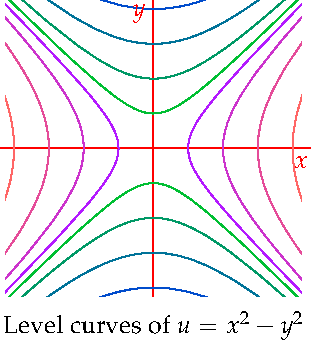
\includegraphics{functions-zsq}
	\end{minipage}
	\goodbreak
	
	%Away from the origin, $f(\pm z)=z^2$ shows that $f$ is a \emph{two-to-one} function.
	The polar form allows us to think about the what $f$ does to the argument:
	\[
		f(z)=r^2e^{2i\theta}\implies \arg f(z)=2\arg z
	\]
	Given a \textcolor{Green}{sector} between arguments $\theta$ and $\phi$, the function \emph{doubles} this to the \textcolor{blue}{sector} between $2\theta$ and $2\phi$. This can also be visualized pathwise. If $z$ traces a \textcolor{Green}{path} which once encircles the origin, then the \textcolor{blue}{path} traced by $z^2$ orbits the origin \emph{twice}. The colored dots on the two paths correspond under $\textcolor{Green}{z}\mapsto \textcolor{blue}{z^2}$.
	\begin{center}
		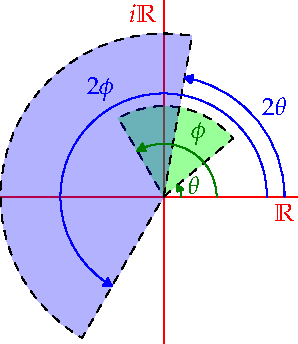
\includegraphics{functions-zsq2}
		\qquad\qquad
		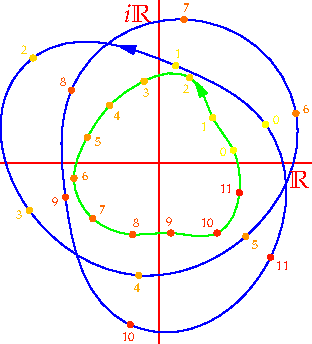
\includegraphics{functions-zsq3}
	\end{center}
\end{example}

	Similar behavior occurs with higher powers. For instance, $z\mapsto z^3$ maps a single loop round the origin to a \emph{triple} loop. %; away from the origin we have a \emph{three-to-one} function. 
	By contrast, the principal square root function $\sqrt z=\sqrt r\polar{i\theta}2$ \emph{halves} the principal argument: $\Arg\sqrt z\in (-\frac\pi 2,\frac\pi 2]$. In the fractional-exponent language of Section \ref{sec:roots},
	\[
		z\mapsto z^{1/2} =\{\sqrt r\polar{i\theta}2,-\sqrt r\polar{i\theta}2\}
	\]
	This is sometimes called a \emph{two-valued} function---we'll return to such objects in Chapter \ref{chap:functions}.


\boldsubsubsection{2D geometry with complex numbers}\phantomsection\label{pg:2dgeom}

Complex functions easily describe the basic geometric transformations of the plane.
\begin{description}
	\item[Translation] If $w$ is constant, the function $f(z)=z+w$ translates the plane, shifting the origin to $w$.
	\item[Scaling] If $R>0$ is a real constant, the function $f(z)=Rz$ scales/stretches the complex plane relative to the origin.
	\item[Rotation] Given $\phi\in\R$, the function $f(z)=e^{i\phi}z$ rotates the plane by $\phi$ radians counter-clockwise around the origin. This is easy to see in polar form:
	\[
		f(z)=f(re^{i\theta})=e^{i\phi}re^{i\theta}=re^{i(\theta+\phi)}
	\]
	\item[Reflection] Complex conjugation $f(z)=\cl z=x-iy$ reflects the plane in the horizontal axis.
\end{description}

By composing such functions, we can describe arbitrary rotations, reflections and scalings relative to any points/lines.



\begin{examples}{}{analyticpg2}
	\exstart We construct rotation by $\frac\pi 3=\ang{60}$ counter-clockwise about $2i$ in three stages:
	\begin{enumerate}\setcounter{enumi}{1}
	  \item[]\begin{enumerate}
	  	\item Translate $2i$ to the origin: \ $z\mapsto z-2i$
	  	\item Rotate by $\frac\pi 3$ about the origin: \ $z\mapsto e^{\frac{i\pi}3}(z-2i)$
	  	\item Translate the origin back to $2i$: \ $z\mapsto f(z) =\polar{i\pi}3(z-2i)+2i$
		\end{enumerate}
	  
		\item We may similarly produce any reflection. To reflect in the line through 0 and $w$ with $\Arg w=\phi$;
		\begin{enumerate}
		  \item Rotate the plane by $-\phi$: \ $z\mapsto e^{-i\phi}z$
		  \item Reflect in the real axis: \ $z\mapsto \cl{e^{-i\phi}z}=e^{i\phi}\cl z$
		  \item Rotate the plane back by $\phi$: \ $z\mapsto f(z)=e^{2i\phi}\cl z$
		\end{enumerate}
	  
	  \item\label{ex:reflect2} We compute the function that reflects across the line joining $\alpha=2+i$ and $\beta=4+3i$.\smallbreak
	  Since $\beta-\alpha=2+2i$ has argument $\phi=\frac\pi 4$, we combine reflection across the line making $\phi$ through the origin with translation by $\alpha$ (translate by $-\alpha$, reflect, translate back by $\alpha$):
	  \begin{align*}
		  f(z)&=e^{2i\phi}(\cl{z-\alpha})+\alpha =\polar{i\pi}2(\cl{z-2-i})+2+i=i(\cl z-2+i)+2+i\\
		  &=i\cl z+1-i
	  \end{align*}
	  As a sanity check, you should verify explicitly that $f(\alpha)=\alpha$ and $f(\beta)=\beta$: why?
	\end{enumerate}
\end{examples}


\begin{exercises*}
	\exstart For each function, describe its implied domain (page \pageref{sec:func}).
	\begin{enumerate}\setcounter{enumi}{1}
	  \item[]\begin{enumerate}
	    \item $\displaystyle f(z)=\frac 1{4+z^2}$\qquad
	    (b) \ $\displaystyle f(z)=\frac{z-1}{e^z-1}$\qquad
	    (c) $\displaystyle f(z)=\frac{z^2+z+1}{z^4-1}$
	  \end{enumerate}
	  
	  \item Write the function in terms of its real and imaginary parts: $f(z)=u(x,y)+iv(x,y)$.
	  \begin{enumerate}
	  	\item $\displaystyle f(z)=z^3-4z^2+2$\qquad
	    (b) \ $\displaystyle f(z)=\frac{z^2}{1-\cl z}$\qquad
	    (c) $\displaystyle f(z)=e^{\cl z}$
	  \end{enumerate}
	  
	  \item Write the function $\displaystyle f(z)=\frac 1{\nm z^2}\cl z$ in polar form.
	  
	  \item Find an expression for the function which reflects across the vertical line through $\alpha=-1$.
	  
	  \item In Example \ref*{ex:analyticpg2}.\ref{ex:reflect2}, evaluate the function $\displaystyle g(z)=e^{2i\phi}(\cl{z-\beta})+\beta$. Why are you not surprised by the result?
	  
	  \item Let $\phi=\tan^{-1}\frac 34$. Find the result (in rectangular co-ordinates) of rotating $z=-2+i$ counter-clockwise by $\phi$ radians around the origin.\par
	  (\emph{Hint: consider a 3:4:5 triangle!})
	  
	  \item Prove, using the expressions on page \pageref{pg:2dgeom}, that the composition of two reflections is a rotation, and that the composition of a rotation and a reflection is a reflection.
	\end{enumerate}
\end{exercises*}
\clearpage



\subsection{Open sets, Limits and Continuity}

Before we can differentiate, we need to understand limits and continuity. We start by reviewing several preliminaries without proof. Almost all of this is identical to (multivariable) real analysis.

\begin{defn}{Sequences and Limits}{}{}
	Let $(z_n)=(z_1,z_2,\ldots)$ be a \emph{sequence} of complex numbers.
	\begin{enumerate}\itemsep2pt
	  \item $(z_n)$ \emph{converges} to $z_0$, and we write \smash[b]{$\lim\limits_{n\to \infty}z_n=z_0$} or simply $z_n\to z_0$, if
		\[
			\forall \epsilon>0,\ \exists N\text{ such that }n>N\implies \nm{z_n-z_0}<\epsilon
		\]
		
		\item $(z_n)$ is a \emph{Cauchy sequence} if
		\[
			\forall \epsilon>0,\ \exists N\text{ such that }m,n>N\implies \nm{z_m-z_n}<\epsilon
		\]
	\end{enumerate}
\end{defn}

\begin{thm}{}{}
	\exstart Cauchy completeness: $(z_n)$ converges if and only if it is Cauchy.
	\begin{enumerate}\setcounter{enumi}{1}
	  \item Bolzano--Weierstraß: If $(z_n)$ is bounded, then it has a convergent subsequence.
	\end{enumerate}
\end{thm}

\begin{defn}{Disks, Sets and Neighborhoods}{disks}
	The \emph{\textcolor{Green}{open disk}} (or \emph{$\delta$-ball}) centered at $z_0\in\C$ with radius $\delta$ is the set\par
	\begin{minipage}[t]{0.65\linewidth}\vspace{-12pt}
		\[
			B_\delta(z_0)=\{z\in\C:\nm{z-z_0}<\delta\}
		\]
		For the \emph{punctured open disk}, remove the central point $z_0$:
		\[
			\{z\in\C:0<\nm{z-z_0}<\delta\}
		\]
		Let $D\subseteq \C$ be a subset.
	\end{minipage}
	\hfill
	\begin{minipage}[t]{0.3\linewidth}\vspace{-16pt}
		\centering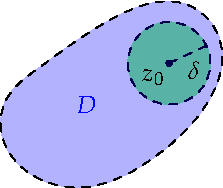
\includegraphics{functions-open}\\
		An open neighborhood of $z_0$
	\end{minipage}
	\par\vspace{-5pt}
	\begin{itemize}\itemsep2pt
		\item $D$ is \emph{open} if every point is \emph{interior}: at every point we can center an open disk $B_\delta(z_0)\subseteq D$:
		\[
			\forall z_0\in D, \ \exists \delta>0\text{ such that } \nm{z-z_0}<\delta\implies z\in D
		\]
		%\vspace{-20pt}
		\item $D$ is a \emph{neighborhood} of $z_0$ if it contains some $B_\delta(z_0)$. A neighborhood can, but need not, be open. A \emph{punctured neighborhood} instead contains a punctured disk.
		\item $D$ is \emph{closed} if its complement $\C\setminus D$ is open.
	\end{itemize}
\end{defn}

\begin{thm}{}{}
	$K$ is closed if and only if every Cauchy sequence $(z_n)\subseteq K$ has its limit in $K$.
\end{thm}

%We define continuity of functions in the usual way.

\begin{defn}{Continuity}{contdef}
	Let $f:D\to\C$ and $z_0\in D$. We say that $f$ is \emph{continuous at $z_0$} if
	\[
		\forall \text{ sequences } (z_n)\subseteq D\text{ with }z_n\to z_0\text{ we have }f(z_n)\to f(z_0)
	\]
	$f$ is \emph{continuous} (on $D$) if it is continuous at all points $z_0\in D$.
\end{defn}

\goodbreak

As in real analysis, it is helpful to relate continuity to limits of functions.

\begin{defn}{Limits of Functions}{limit}
	Let $f:D\to\C$, where $D$ contains an open punctured neighborhood of $z_0$. We say that $w_0$ is the \emph{limit of $f$ as $z$ approaches $z_0$} and write $\lim\limits_{z\to z_0}f(z)=w_0$, if
	\[
		\forall \epsilon>0,\ \exists \delta>0\text{ such that } 0<\nm{z-z_0}<\delta\implies \nm{f(z)-w_0}<\epsilon
	\]
\end{defn}

\begin{thm}{}{}
	Let $z_0$ be an \emph{interior} point of $D$. Then $f:D\to\C$ is continuous at $z_0$ if and only if
	\[
		\lim\limits_{z\to z_0}f(z)=f(z_0)
	\]
\end{thm}

Otherwise said, for any $\epsilon$-ball $B_\epsilon\bigl(f(z_0)\bigr)$, there exists a $\delta$-ball $B_\delta(z_0)$ such that $f\bigl(B_\delta(z_0)\bigr)\subseteq B_\epsilon\bigl(f(z_0)\bigr)$.
\smallbreak


We won't spend much time on calculations since these tend to proceed similarly to real analysis.

\begin{example}{}{}
	We show that $f(z)=z^2$ is continuous (on $\C$) by proving that $\lim\limits_{z\to z_0}z^2=z_0^2$ for all $z_0$.\smallbreak
	Let $z_0\in\C$ and $\epsilon>0$ be given. Define $\delta=\min\{1,\frac\epsilon{1+2\nm{z_0}}\}$. By the triangle-inequality,
	\[
		\nm{z-z_0}<\delta\implies \nm{z+z_0}=\nm{z-z_0+2z_0}\le \nm{z-z_0}+2\nm{z_0}<\delta+2\nm{z_0}\le 1+2\nm{z_0}
	\]
	from which
	\[
		\nm{z-z_0}<\delta\implies \nm{z^2-z_0^2}=\nm{z-z_0}\nm{z+z_0}<\delta(1+2\nm{z_0})\le \epsilon
	\]
	The picture below should help you visualize things. Given an \textcolor{blue}{$\epsilon$-ball} centered at $w_0=z_0^2$, we've described how to choose $\delta>0$ so that $f$ maps the \textcolor{Green}{$\delta$-ball} centered at $z_0$ to a \textcolor{Green}{region} \emph{inside} the original \textcolor{blue}{$\epsilon$-ball.}
	\begin{center}
		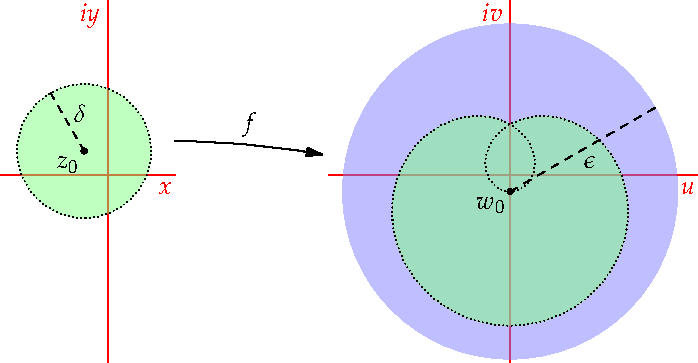
\includegraphics{limits-zsq}
	\end{center}
	The picture illustrates the case when
	\[
		z_0=\frac 12\polar{3\pi i}4=\frac 1{2\sqrt 2}(-1+i),\quad w_0=-\frac i4,\quad \epsilon=\frac 52\quad\text{and}\quad \delta=\min\left\{1,\tfrac{5/2}{1+2\cdot\frac 12}\right\}=1
	\]
\end{example}
\goodbreak


\begin{thm}{Basic Limit Results}{basiclimit}
Let $f,g:D\to\C$ be functions and $z_0=x_0+iy_0$ be a point satisfying the assumptions of Definition \ref{defn:limit}.
\begin{enumerate}
  \item Limits are unique: If $w_0$ and $\widetilde{w_0}$ satisfy Definition \ref{defn:limit}, then $\widetilde{w_0}=w_0$.
  \item\label{thmbaslim2} If $f(z)=u(x,y)+iv(x,y)$ and $w_0=u_0+iv_0$, then
  \[
  	\lim_{z\to z_0}f(z)=w_0\iff \lim_{(x,y)\to (x_0,y_0)}\hspace*{-10pt} u(x,y)=u_0\quad \text{and}\quad \lim_{(x,y)\to (x_0,y_0)}\hspace*{-10pt} v(x,y)=v_0
  \]
  In particular $\lim\limits_{z\to z_0}\cl z=\cl{z_0}$
  \item Suppose $\lim\limits_{z\to z_0}f(z)=w_0$ and $\lim\limits_{z\to z_0}g(z)=w_1$:
  \begin{enumerate}
    \item For any $a,b\in\C$, $\lim\limits_{z\to z_0}\bigl( af(z)+bg(z)\bigr)=aw_0+bw_1$
    \item $\lim\limits_{z\to z_0}\bigl(f(z)g(z)\bigr)=w_0w_1$
    \item $\lim\limits_{z\to z_0}\frac{f(z)}{g(z)}=\frac{w_0}{w_1}$, provided $w_1\neq 0$ and $g(z)\neq 0$ on a punctured neighbourhood of $z_0$.
    \item If $h$ is a function such that $\lim\limits_{w\to w_0}h(w)=w_2$, then $\lim\limits_{z\to z_0}h(f(z))=w_2$
	\end{enumerate}
\end{enumerate}
\end{thm}

The basic limit laws should feel familiar and intuitive; indeed analogues of most should have been proved in real analysis. Parts 2 \& 3 have obvious corollaries for continuous functions. For instance:

\begin{cor}{}{}
	$f:D\subseteq\C\to\C$ is continuous if and only if its real and imaginary parts $u,v:D\to\R$ are also continuous. 
\end{cor}

Several pieces of part 3 follow from part 2 by considering real and imaginary parts and the limit laws for functions $\R^2\to\R$. For instance, write $f(z)=u_1+iv_1$ and $g(z)=u_2+iv_2$, then
\[
	\lim\limits_{z\to z_0}\bigl(f(z)g(z)\bigr) =\lim\limits_{z\to z_0}\bigl(u_1u_2-v_1v_2+i(u_1v_2+v_1u_2)\bigr) =w_0w_1
\]

\begin{examples}{}{}
	\exstart $\lim\limits_{z\to 1+3i}(z^2-i\cl z) =(1+3i)^2-i\bigl(\cl{1+3i}\bigr) =1+6i-9-i(1-3i)=-11+5i$.
	\begin{enumerate}\setcounter{enumi}{1}
	  \item Every polynomial function is continuous on $\C$.
	  \item Every rational function $f(z)=\frac{p(z)}{q(z)}$ (where $p,q$ are polynomials), is continuous on its implied domain $D=\{z:q(z)\neq 0\}$.
	  \item The exponential function
	  \[
	  	\exp(z)=e^z=e^xe^{iy}=e^x\cos y+ie^x\sin y
	  \]
	  is continuous on $\C$, since the exponential, cosine and sine are continuous on $\R$.
	\end{enumerate}
\end{examples}

\vfil\goodbreak


\boldsubsubsection{Limits and the Point at Infinity}

In (single-variable) real analysis there are \emph{two} infinities ($\pm\infty$). In complex analysis, the convention is to have only one: for instance, the sequences $z_n=n$ and $w_n=in$ both diverge to the \emph{same} infinity.

\begin{defn}{}{rsphere}
	The \emph{extended complex plane} (\emph{Riemann sphere}) is the set $\cl\C=\C\cup\{\infty\}$ where $\infty$ denotes the \emph{point at infinity.} The concepts of neighborhood, openness and limit extend to the point at infinity:
	\begin{enumerate}
	  \item A \emph{neighborhood} of $\infty$ is any set containing an \emph{open disk} at $\infty$; a subset of the form
		\[
			\{\infty\}\cup\{z\in\C:\nm{z}>M\}
		\]
	  \item $\lim\limits_{z\to z_0}f(z)=\infty$ means: $\forall M>0$, $\exists \delta>0$ such that $0<\nm{z-z_0}<\delta \implies \nm{f(z)}>M$
	  \item $\lim\limits_{z\to \infty}f(z)=w_0$ means: $\forall \epsilon>0$, $\exists N>0$ such that $\nm{z}>N \implies \nm{f(z)-w_0}<\epsilon$
	  \item $\lim\limits_{z\to\infty}f(z)=\infty$ means: $\forall M>0$, $\exists N>0$ such that $\nm{z}>N\implies \nm{f(z)}>M$
	\end{enumerate}
\end{defn}

\begin{example}{}{}
	We verify that $\lim\limits_{z\to -3i}\frac{z^2}{z+3i}=\infty$. Let $M>0$ be given and define $\delta=\min\{1,\frac 4{M}\}$. Then
  \begin{align*}
  	0<\nm{z+3i}<\delta&\implies \nm z\ge \nm{3i}-\nm{z+3i}>3-\delta\ge 2\\
  	&\implies\nm{\frac{z^2}{z+3i}} > \frac{4}{\delta} \ge M
  \end{align*}
\end{example}


The relationship between limits, zero and infinity feel like the dubious claims $\frac 1\infty=0$ and $\frac 10=\infty$!

\begin{thm}{}{infty}
	Provided all limits make sense, Theorem \ref{thm:basiclimit} also applies to limits involving infinity. Moreover, we have the additional relationships:
	\begin{enumerate}
	  \item $\lim\limits_{z\to z_0}f(z)=\infty \iff \lim\limits_{z\to z_0}\frac 1{f(z)}=0$ \qquad\qquad 2.\ \ $\lim\limits_{z\to\infty}f(z)=w_0 \iff \lim\limits_{z\to 0}f\left(\frac 1z\right)=w_0$
	  \setcounter{enumi}{2}
	  \item $\lim\limits_{z\to \infty}f(z)=\infty \iff \lim\limits_{z\to 0}\frac 1{f(1/z)}=0$
	\end{enumerate}
\end{thm}

\begin{proof}[Sketch Proof]
	Suppose $\lim\limits_{z\to\infty}f(z)=w_0$. Let $\delta=\frac 1N$ to see that
	\[
		\forall \epsilon>0,\exists \delta>0\text{ such that }0<\tfrac 1z<\delta \implies \nm{f(\tfrac 1z)-w_0}<\epsilon
	\]
	The other five results are similar.
\end{proof}


\begin{example}{}{}
	Consider $f(z)=\frac{5iz+1}{3z-2i}$. Plainly 
  \begin{gather*}
  	\lim_{z\to\frac 23i}\frac 1{f(z)}=\lim_{z\to\frac 23i}\frac{3z-2i}{5iz+1}=0\implies \lim_{z\to\frac 23i}f(z)=\infty\\
  	\lim_{z\to\infty}f(z)= \lim_{z\to\infty}\frac{5i+1/z}{3-2i/z} = \frac{5i+\lim\frac 1z}{3-2i\lim\frac 1z}=\frac 53i
  \end{gather*}\goodbreak
% The function $f(z)=\frac 1z$ is a continuous bijection $f:\cl\C\to\cl\C$ satisfying $f(0)=\infty$ and $f(\infty)=0$: indeed it is its own inverse! We can show directly that $f$ is continuous at zero: given $M>0$, let $\delta=\frac 1M$ to see that
% \[\nm{z-0}<\delta\implies \nm z<\frac 1M\implies \nm{f(z)}=\frac 1{\nm z}>M\]
% whence $\lim\limits_{z\to 0}f(z)=\infty=f(0)$.
% \begin{enumerate}\setcounter{enumi}{1}
%   \item Consider $f(z)=\frac{5iz+1}{3z-2i}$. Since
%   \[\lim_{z\to\frac 23i}f(z)=\infty\quad\text{and}\quad \lim_{z\to\infty}f(z)= \lim_{z\to\infty}\frac{5i+1/z}{3-2i/z}=\frac 53i\]
%   we can consider $f$ as a function $f:\cl\C\to\cl\C$ satisfying $f\left(\frac 23i\right)=\infty$ and $f(\infty)=\frac 53i$. 
% \end{enumerate}
Because of these calculations, it is common to view $f$ as a continuous bijection $f:\cl\C\to\cl\C$ of the Riemann sphere with itself (exercise):
\[
	f(z):=
	\begin{cases}
		\frac{5iz+1}{3z-2i}&\text{if }z\neq \frac 23i,\infty\\
		\infty&\text{if }z=\frac 23i\\
		\frac 53i&\text{if }z=\infty
	\end{cases}
\]
\end{example}

\begin{aside}{\bf Aside (non-examinable)}{}
	The Riemann sphere is merely a fun diversion for us. Unless indicated otherwise, all sets should be assumed to be subsets of the (\emph{finite}) complex plane.\par
	\begin{minipage}[t]{0.49\linewidth}\vspace{-5pt}
		The Riemann sphere is so-named because it can be visualized as a \textcolor{blue}{sphere $S^2$}, with $\infty$ playing the role of the north pole. The rest of the sphere is identified bijectively with the \textcolor{Green}{equatorial plane $\C$} via \href{https://en.wikipedia.org/wiki/Stereographic_projection}{\emph{stereographic projection}} $\pi:S^2\to\cl\C$. In the picture, the image of $P\in S^2$ is the intersection $\pi(P)$ of $\C$ with the line through $P$ and $N=\pi^{-1}(\infty)$.
	\end{minipage}
	\hfill
	\begin{minipage}[t]{0.5\linewidth}\vspace{0pt}
		\flushright%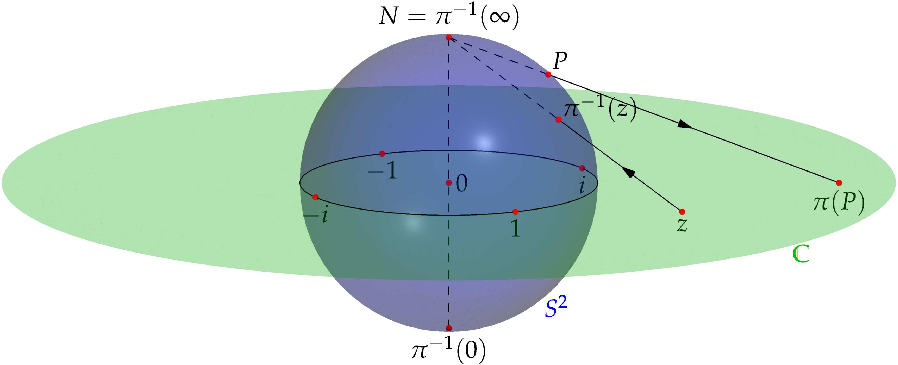
\includegraphics{complex-stereo+0_0}
		\href{https://www.math.uci.edu/~ndonalds/math147/complex-stereo.html}{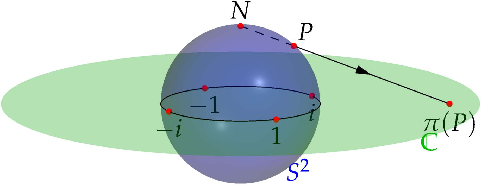
\includegraphics{complex-stereo}}
	\end{minipage}
\end{aside}

 
\boldsubsubsection{Compactness, Path-Connectedness \& Continuity}

We finish with two further desirable properties of domains.

\begin{defn}{}{}
	\exstart A subset $K\subseteq\C$ is \emph{compact} if it is closed and bounded.
	\begin{enumerate}\setcounter{enumi}{1}
	  \begin{minipage}[t]{0.6\linewidth}\vspace{0pt}
	  	\item $K\subseteq\C$ is \emph{path-connected} if any two points can be joined by a path lying entirely within $K$: more precisely, $\forall p,q\in K$,
	  	\[
	  		\exists z:[0,1]\to K \text{ continuous } \text{ with }
	  z(0)=p \text{ and }z(1)=q
	  	\]
	  \end{minipage} 
	  \begin{minipage}[t]{0.39\linewidth}\vspace{-12pt}
			\flushright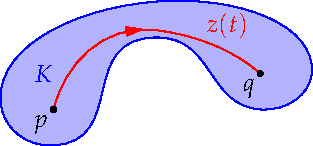
\includegraphics[scale=1]{limits-topology}
	  \end{minipage} 
	\end{enumerate} 
\end{defn}

These concepts generalize notions of intervals from single-variable real analysis. In view of this, we translate two familiar results, essentially the \emph{extreme} and \emph{intermediate value theorems} of real analysis.

\begin{thm}{}{compactconnected}
	Suppose $f:K\to\C$ is continuous.
	\begin{enumerate}
  	\item If $K$ is compact, so is the image $f(K)$.
  	\item If $K$ is path-connected, so is $f(K)$.
	\end{enumerate}
\end{thm}

\begin{proof}{}{}
	\begin{enumerate}
	  \item Consider the \emph{real-valued} function $\nm{f}$ and apply the same argument from real analysis:
		\begin{itemize}
		  \item Let $M=\sup\{\nm{f(z)}:z\in K\}$. Then $\exists (z_n)\subseteq K$ such that $\lim\nm{f(z_n)} =M$.
		  \item $K$ is bounded; Bolzano--Weierstraß says $(z_n)$ has a convergent subsequence $(z_{n_k})$.
		  \item Let $z_0=\lim z_{n_k}$. Since $K$ is closed, we have $z_0\in K$, whence $f(z_0)$ is defined.
		  \item $f$ continuous $\Longrightarrow\lim f(z_{n_k})= f(z_0)$; thus $M=f(z_0)$ is finite and $f(K)$ is bounded.
		  \item The closure of $f(K)$ is a short exercise.
		  %Now suppose $(w_n)$ is a sequence in $K$ such that $(f(w_n))$ is convergent in $\C$. The compactness of $K$ says $\exists (w_{n_k})$ convergent to $w\in K$. The continuity of $f$ says that $f(w_{n_k})\to f(w)$. $f(K)$ is therefore closed.
		\end{itemize}
		\item This is also an exercise.\qedhere %Suppose $f(p),f(q)\in f(K)$ and let $z:[0,1]\to K$ be a path from $p$ to $q$. Then  $w(t):=f(z(t))$ defines a path from $f(p)$ to $f(q)$ in $f(K)$.
	\end{enumerate}
\end{proof}

\goodbreak

Later on we'll need one final fact about compactness, which we again state without proof.

\begin{thm}{}{opencover}
	Let $K$ be compact and suppose that a collection of open sets $U_j$ satisfies $K\subseteq \smash[b]{\bigcup\limits_{j\in I} U_j}$.\par
	Then there exists a \underline{finite} subset $J\subseteq I$ such that $K\subseteq \bigcup\limits_{j\in J} U_j$.
\end{thm}

This is usually said ``Every open cover has a finite subcover,'' and is taken, in topology, as the definition of compactness. That this is equivalent to being closed and bounded in $\C$ (or any Euclidean space) is the famous Heine--Borel Theorem.


\begin{exercises*}{}{}
	\exstart Use the $\epsilon$--$\delta$ definition (\ref{defn:limit}) to prove the following.
	\begin{enumerate}\setcounter{enumi}{1}
	  \item[]\begin{enumerate}
	  	\item $\displaystyle\lim\limits_{z\to z_0}\cl z=\cl{z_0}$\qquad
	  	(b) \ $\displaystyle\lim\limits_{z\to 0}\frac{\cl z^2}z=0$\qquad
	  	(c) \ $\displaystyle\lim\limits_{z\to 2}\frac 1{z-i}=\frac 1{2-i}$\qquad
	  	(d) \ $\displaystyle\lim\limits_{z\to z_0}z^3=z_0^3$
	  \end{enumerate}
	  
	  
	  \item Show that the function $f(z)=\left(\dfrac z{\cl z}\right)^2$ ($\cl z$ in the denominator!) has value 1 at all non-zero points on the real and imaginary axes, and $-1$ at all non-zero points on the line $y=x$. Hence explain why $\lim\limits_{z\to 0}f(z)$ does not exist.
	  
	  
	  \item Prove part 3(c) of Theorem \ref{thm:basiclimit}.
	  
	  
	  \item Suppose $\lim\limits_{z\to z_0}f(z)=w_0$. Prove that $\lim\limits_{z\to z_0}\nm{f(z)}=\nm{w_0}$.
	   
	   
	  \item Use Definition \ref{defn:rsphere} to prove part of Theorem \ref{thm:infty}: $\lim\limits_{z\to z_0}f(z)=\infty \implies \lim\limits_{z\to z_0}\frac 1{f(z)}=0$.
	  
	  
	  \item Use Definition \ref{defn:rsphere} to prove that
	  \begin{enumerate}
	    \item $\displaystyle\lim\limits_{z\to 2i}\frac{iz-1}{z-2i}=\infty$ \qquad (b) \ $\displaystyle\lim\limits_{z\to\infty}\frac{iz-1}{z-2i}=i$.
	  \end{enumerate}
	  
	  
	 	\item\begin{enumerate}
	    \item Show that $f(z)=\dfrac{5iz+1}{3z-2i}$ defines a bijection of the Riemann sphere $f:\cl\C\to\cl\C$.\par
	  	(\emph{Hint: let $w=f(z)$ and solve for $z\ldots$})
	  	
	  	\item More generally, given complex numbers $\alpha,\beta,\gamma,\delta$, consider $f(z)=\dfrac{\alpha z+\beta}{\gamma z+\delta}$.\par
	  	Prove that this defines a bijection of the Riemann sphere if and only if $\alpha\delta-\beta\gamma\neq 0$. How does this discussion relate to the $2\times 2$ matrix $\begin{smatrix}\alpha&\beta\\\gamma&\delta\end{smatrix}$?
	  \end{enumerate}
	  
	  
	  \item We complete the proof of Theorem \ref{thm:compactconnected}. Suppose $f:K\subseteq\C\to\C$ is continuous.
	  \begin{enumerate}
	    \item Let $K$ be compact. Suppose $(w_n)\subseteq K$ is a sequence such that $\bigl(f(w_n)\bigr)$ is convergent in $\C$. Explain why there exists a convergent subsequence $(w_{n_k})$, and use it to show that $\lim f(w_n)\in f(K)$. Hence conclude that $f(K)$ is closed.
	    % such that $f(w_{n_k})$ Use the Bolzano--Weierstrass theorem  The compactness of $K$ says $\exists (w_{n_k})$ convergent to $w\in K$. The continuity of $f$ says that $f(w_{n_k})\to f(w)$. $f(K)$ is therefore closed.
			\item Suppose $K$ is path-connected. If $f(p),f(q)\in f(K)$, show that $\exists w:[0,1]\to f(K)$ continuous such that $w(0)=f(p)$ and $w(1)=f(q)$. Hence conclude that $f(K)$ is path-connected.
			% and let $z:[0,1]\to K$ be a path from $p$ to $q$. Then  $w(t):=f(z(t))$ defines a path from $f(p)$ to $f(q)$ in $f(K)$.
	  \end{enumerate}
	\end{enumerate}
\end{exercises*}

\clearpage


\subsection{Derivatives \& the Cauchy--Riemann Equations}% (\S\,19-23)

Differentiation is where complex analysis shows significant differences from real analysis, though it won't appears so at first, since the definition of derivative is exactly what you are used to.

\begin{defn}{}{deriv}
Let $f:D\to\C$ be a complex function and $z_0$ an \emph{interior} point of $D$. We say that $f$ is \emph{differentiable at $z_0$} if the following limit exists.
\[\lim_{z\to z_0}\frac{f(z)-f(z_0)}{z-z_0}\]
We call this limit the \emph{derivative} of $f$ at $z_0$ and denote it by $f'(z_0)$. If $f$ is differentiable everywhere\footnote{Such \emph{holomorphic} functions are the main topic of the course: we'll consider them more properly in the next section. Necessarily, $D$ must be an open set if $f$ is to be holomorphic (think about the definition of the limit!).} on $D$ then the derivative is a function; $f'(z)$ or $\diff[f]{z}$. 
\end{defn}

As with limits, we quickly consider an easy example and record the basic facts.

\begin{example}{}{}
The function $f(z)=z^2$ is everywhere differentiable,\footnote{Remember that when taking limits, we only compute on a punctured disk $0<\nm{z-z_0}<\delta$, hence the \textcolor{red}{red} equality.}
  \[\lim_{z\to z_0}\frac{f(z)-f(z_0)}{z-z_0}= \lim_{z\to z_0}\frac{z^2-z_0^2}{z-z_0} =\lim_{z\to z_0}\frac{(z-z_0)(z+z_0)}{z-z_0} \textcolor{red}{\,=\,} \lim_{z\to z_0}z+z_0=2z_0\]
\end{example}

The basic rules of differentiation are identical those in real analysis and can be proved similarly. We state them for reference.

\begin{thm}{}{derivrules}
Suppose $f$ and $g$ are differentiable (either at a point $z_0$ or as functions).
\begin{enumerate}
  \item (Linearity)\quad For any constants $a,b\in\C$, $\displaystyle\diff z(af(z)+bg(z))=af'(z)+bg'(z)$
  \item (Power Law)\quad For any $n\in\N_0$, $\displaystyle\diff zz^n=nz^{n-1}$
  \item (Product rule)\quad $\displaystyle\diff z(f(z)g(z))=f'(z)g(z)+f(z)g'(z)$
  \item (Quotient Rule)\quad If $g(z)\neq 0$, then $\displaystyle\diff z\frac{f(z)}{g(z)}=\frac{f'(z)g(z)-f(z)g'(z)}{[g(z)]^2}$
  \item (Chain Rule)\quad If $h$ is differentiable at $g(z_0)$, then $h\circ g$ is differentiable at $z_0$ and
  \[(h\circ g)'(z_0)=h'\bigl(g(z_0)\bigr)g'(z_0)\]
\end{enumerate}
\end{thm}

We immediately see that all polynomials and rational function are differentiable. Indeed we can easily compute familiar examples without caring whether we are in $\R$ or $\C$!
\begin{example}{}{}
  $\displaystyle\diff z\frac{3(z^2-2)^5+z^2}{z^3+1} = \frac{[30z(z^2-2)^4+2z)](z^3+1) -3z^2[3(z^2-2)^5+z^2]}{(z^3+1)^2}$
\end{example}


\vfil\goodbreak

\boldsubsubsection{The Cauchy--Riemann Equations}


Thus far, differentiation seems uncontroversial. Here is example that might change your mind\ldots

\begin{example}{}{}
Consider the complex conjugate function $f(z)=\cl z$. We attempt to compute the limit
  \[\lim\limits_{z\to z_0}\frac{f(z)-f(z_0)}{z-z_0}=  \lim\limits_{(x,y)\to(x_0,y_0)} \frac{x-iy-x_0+iy_0}{x+iy-x_0-iy_0} = \lim\limits_{(\Delta x,\Delta y)\to (0,0)} \frac{\Delta x-i\Delta y}{\Delta x+i\Delta y}\]
  
  \begin{minipage}[t]{0.7\linewidth}\vspace{0pt}
  For $f'(z)$ to exist, we must obtain the same value \emph{regardless of how $(\Delta x,\Delta y)\to (0,0)$.} There are two obvious ways to take the limit:
  \begin{itemize}
  \item[]\normalfont\emph{\textcolor{blue}{Horizontally}}\quad $\displaystyle\Delta y=0\implies \frac{f(z)-f(z_0)}{z-z_0} =1$
  \item[]\normalfont\emph{\textcolor{Green}{Vertically}}\quad $\displaystyle\Delta x=0\implies \frac{f(z)-f(z_0)}{z-z_0} =-1$
  \end{itemize}
  \end{minipage}\begin{minipage}[t]{0.3\linewidth}\vspace{-5pt}
  \flushright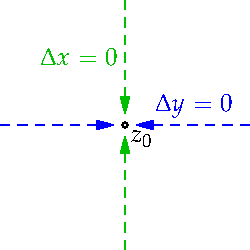
\includegraphics{diff-cr}  
  \end{minipage}\par
  The quotient takes different values depending on how $(\Delta x,\Delta y)\to(0,0)$. We conclude that $f'(z_0)$ \emph{does not exist,} and that the function $f(z)=\cl z$ is not differentiable anywhere!
\end{example}

If the example doesn't surprise you, read it again. There is barely a simpler complex-valued function than the complex conjugate, yet this is not differentiable! We now extend the approach to consider (non-)differentiability more generally.\smallbreak

Let $f(z)=u(x,y)+iv(x,y)$ be written in terms of its real and imaginary parts. As before, we write $z=x+iy$, $z_0=x_0+iy_0$ and denote the differences by
\[\Delta z=z-z_0=\Delta x+i\Delta y =(x-x_0)+i(y-y_0)\]
We attempt to evaluate the limit of the difference quotient
\[\lim\limits_{z\to z_0}\frac{f(z)-f(z_0)}{z-z_0}= \lim\limits_{(\Delta x,\Delta y)\to (0,0)}\frac{u(x,y)-u(x_0,y_0)+i(v(x,y)-v(x_0,y_0)}{\Delta x+i\Delta y}\]
If this exists, then we \emph{must} have the same result when evaluating along straight lines  approaching $z_0$ both horizontally and vertically:
\begin{description}
\item[\normalfont\emph{Horizontally}]\quad We have $\Delta y=0$ and so the limit becomes
\[\lim_{\Delta x\to 0}\frac{u(x,y_0)-u(x_0,y_0)+i(v(x,y_0)-v(x_0,y_0)}{\Delta x} =\left(\partials[u]{x}+i\partials[v]{x}\right)(x_0,y_0)\]
where we see the \emph{partial derivatives} of the functions $u$ and $v$.
\item[\normalfont\emph{Vertically}]\quad We have $\Delta x=0$, from which
\[\lim_{\Delta y\to 0}\frac{u(x_0,y)-u(x_0,y_0)+i(v(x_0,y)-v(x_0,y_0)}{i\Delta y} =\frac 1i\left(\partials[u]{y}+i\partials[v]{y}\right)(x_0,y_0)\]
\end{description}
If $f'(z)$ exists, then these limits are equal (to $f'(z)$ itself). We have therefore proved:

\begin{thm}{Cauchy--Riemann equations}{cauchyriemann}
If $f(z)$ is complex-differentiable, then the real and imaginary parts of $f$ satisfy the \emph{Cauchy--Riemann equations}
\[\partials[u]{x}=\partials[v]{y}\qquad \partials[u]{y}=-\partials[v]{x} \qquad\text{ equivalently}\quad u_x=v_y,\quad u_y=-v_x\]
In such a situation, we can write
\[f'(z)=u_x+iv_x =v_y-iu_y\]
\end{thm}

\begin{examples}{}{crlots}
\hangindent\leftmargini
\textup{1.}\ $f(z)=\cl z=x-iy$ has $u(x,y)=x$ and $v(x,y)=-y$. We quickly see that
  \[u_x=1\neq -1=v_y,\qquad u_y=0=v_x\]
  Since $u,v$ do not satisfy the Cauchy--Riemann equations anywhere (not both of them simultaneously!), $f$ fails to be differentiable anywhere.
\begin{enumerate}\setcounter{enumi}{1}
  \item\label{exs:modnotdiff} $f(z)=\nm z=\sqrt{x^2+y^2}$ has $u=\sqrt{x^2+y^2}$ and $v=0$. The Cauchy--Riemann equations are
  \[u_x=\frac{x}{\sqrt{x^2+y^2}}=0=v_y,\quad u_y=\frac{y}{\sqrt{x^2+y^2}}=0=-v_x\]
  These equations are satisfied nowhere, and so $f(z)$ is nowhere differentiable.\footnote{Note that $u=\sqrt{x^2+y^2}$ isn't even differentiable at $(x,y)=(0,0)$.}
  \item $f(z)=z^2=x^2-y^2+2ixy$ has $u(x,y)=x^2-y^2$ and $v(x,y)=2xy$. We check
  \[u_x=2x=v_y,\qquad u_y=-2y=-v_x\]
  As expected, $u,v$ satisfy the Cauchy--Riemann equations. Moreover,
  \[f'(z)=2z=2x+2iy =u_x+iv_x =v_y-iu_y\]
  
  \item\label{ex:cr3} $\displaystyle f(z)=\frac z{2+\nm z^2}=\frac x{2+x^2+y^2}+\frac{iy}{2+x^2+y^2}$. We compute
  \begin{gather*}
  u_x=\frac{2-x^2+y^2}{(2+x^2+y^2)^2} \qquad v_y=\frac{2+x^2-y^2}{(2+x^2+y^2)^2}\\
  u_y=\frac{-2xy}{(2+x^2+y^2)^2} \qquad -v_x=\frac{2xy}{(2+x^2+y^2)^2}
  \end{gather*}
  The Cauchy--Riemann equations are satisfied if and only if $xy=0=x^2-y^2$, which is if and only if $x=y=0$. We conclude that $f$ is not differentiable at any non-zero $z\in\C$.\smallbreak
  Note that the Cauchy--Riemann equations only provide a \emph{necessary} condition for differentiability. We do not (yet!) have a sufficient condition. However, we can easily check that this function is differentiable at $z=0$, straight from the definition of derivative and the continuity of $\nm z$:
  \[f'(0)=\lim_{z\to 0}\frac{f(z)-f(0)}{z-0}=\lim_{z\to 0}\frac 1{2+\nm z^2}=\frac 12\]
  The function $f$ is therefore differentiable at precisely one point.
\end{enumerate}
\end{examples}

\vfil\goodbreak

\boldsubsubsection{A Sufficient Condition for Differentiability?}

Since Theorem \ref{thm:cauchyriemann} only provides a necessary condition for differentiability, is is most useful in the contrapositive form:
\begin{quote}
Cauchy--Riemann not satisfied $\implies f$ not differentiable 
\end{quote}
We'd like this to be bidirectional, so that the Cauchy--Riemann equations become a sufficient condition for differentiability. This is indeed possible, with one small caveat\ldots\smallbreak

Suppose a complex function $f(z)=u(x,y)+iv(x,y)$ has partial derivatives on an open neighborhood $D$ of a point $z_0=x_0+iy_0$. Also suppose $f$ satisfies the Cauchy--Riemann equations and that the partial derivatives $u_x=v_y$ and $u_y=-v_x$ are \emph{continuous} at $z_0$. The rough idea is to use the linear approximation: for $z\in D$,
\begin{gather*}
\begin{aligned}
f(z)-f(z_0)&\approx f_x(x_0,y_0)\Delta x+f_y(x_0,y_0)\Delta y\\
% &=(u_x(x_0,y_0)+iv_x(x_0,y_0))\Delta x+(u_y(x_0,y_0)+iv_y(x_0,y_0))\Delta y\\
% &=(u_x(x_0,y_0)+iv_x(x_0,y_0))\Delta x+(-v_x(x_0,y_0)+iu_x(x_0,y_0))\Delta y\\
% &=(u_x(x_0,y_0)+iv_x(x_0,y_0))(\Delta x+i\Delta y)\\
&=(u_x+iv_x)\Delta x+(u_y+iv_y)\Delta y\\
&=(u_x+iv_x)\Delta x+(-v_x+iu_x)\Delta y\\
&=(u_x+iv_x)(\Delta x+i\Delta y) =(u_x+iv_x)\Delta z
\end{aligned}\\
\implies \frac{f(z)-f(z_0)}{z-z_0}\approx u_x(x_0,y_0)+iv_x(x_0,y_0) 
\end{gather*}
The continuity of the partial derivatives at $(x_0,y_0)$ means that the approximation approaches equality as $\Delta z\to 0$. We omit the complete proof since there are too many details. The upshot is a near converse to Theorem \ref{thm:cauchyriemann}.

\begin{thm}{}{cauchyriemann2}
Let $u,v$ have partial derivatives on a neighbourhood of $z_0=x_0+iy_0$. Assume $f=u+iv$ satisfies the Cauchy--Riemann equations and has continuous partial derivatives at $z_0$. Then $f$ is differentiable at $z_0$ and
\[f'(z_0)=u_x(x_0,y_0)+iv_x(x_0,v_0)\]
\end{thm}

\begin{examples}{}{crmoremore}
\hangindent\leftmargini
\textup{1.}\ Revisiting Example \hyperref[ex:cr3]{\ref*{ex:crlots}.\ref*{ex:cr3}}, we see that $f(z)=\frac z{2+\nm z^2}$ has partial derivatives everywhere; these are continuous and satisfy Cauchy--Riemann at $z=0$, whence $f$ is differentiable there. Moreover 
  \[f'(0)=u_x(0,0)+iv_x(0,0)=\frac 12\]
\begin{enumerate}\setcounter{enumi}{1}
  \item\label{ex:crexex2} The exponential function is differentiable everywhere: indeed
  \[f(z)=e^z=e^x\cos y+ie^x\sin y\]
  satisfies
  \[u_x=e^x\cos y=v_y,\qquad u_y=-e^x\sin x=-v_x\]
  where these are certainly continuous on $\C$. Moreover, as expected,
  \[f'(z)=u_x+iv_x=e^x\cos y+ie^x\sin y =e^z\]
\end{enumerate}
\end{examples}



\begin{exercises*}{}
\hangindent\leftmargini
\textup{1.}\ Use Theorem \ref{thm:derivrules} to find the derivatives of the following functions:
\begin{enumerate}\setcounter{enumi}{1}
  \item[]\begin{enumerate}
  	\item $\displaystyle f(z)=\frac 1{z^2+2z}$\qquad
    (b) $\displaystyle f(z)=(z^3+2iz+1)^7$\qquad
    (c) $\displaystyle f(z)=\frac{(3z^2-i)^3}{(iz^3+4)^2}$
  \end{enumerate}
  
  \item Use the limit definition of the derivative to compute the derivative of the functions:
  \begin{enumerate}
  	\item $\displaystyle f(z)=3z^3-iz^2$\qquad
    (b) $\displaystyle f(z)=\frac 1{z^2}$
  \end{enumerate}
  
  \item Give a proof of the quotient rule, directly using the definition of the derivative.
  
  \item Use the quotient rule to prove the power law for negative integer exponents: that is
  \[\forall n\in\N,\quad \diff zz^{-n}=-nz^{-n-1}\]
  
  \item Suppose $f(z_0)=g(z_0)=0$ and that $f'(z_0)$ and $g'(z_0)$ exists, where $g'(z_0)\neq 0$. Use the definition of the derivative to show that
  \[\lim_{z\to z_0}\frac{f(z)}{g(z)}=\frac{f'(z_0)}{g'(z_0)}\]
  
  \item Prove that the functions $f(z)=\Re z$ and $g(z)=\Im z$ are not differentiable anywhere.
  
  \item Exactly as in Example \hyperref[ex:crexex2]{\ref*{ex:crmoremore}.\ref*{ex:crexex2}}, prove that $\displaystyle \diff ze^{kz} =ke^{kz}$ for any complex constant $k$.
  
  \item Consider the Cauchy--Riemann equations for the following functions: what can you conclude, if anything?
  \begin{enumerate}
  	\item $\displaystyle f(z)= \frac{1}{\cl z-i}$\qquad
    (b) $\displaystyle f(z)=z^3-\frac 2z$\qquad
    (c) $\displaystyle f(z)=(\nm z^2+z)^2$
  \end{enumerate}
  
  \item Write a complex function $f(z)=f(z,\cl z)$ as a function of $z$ and $\cl z$. For example,
  \[f(z)=\nm z^2=z\cl z\]
  Noting that $\displaystyle x=\frac 12(z+\cl z)$ and $\displaystyle y=\frac 1{2i}(z-\cl z)$, use the chain rule
  \[\partials[f]{\cl z}=\partials[f]{x}\partials[x]{\cl z}+\partials[f]{y}\partials[y]{\cl z}\]
  to prove that $f$ satisfies the Cauchy--Riemann equations if and only if $\displaystyle \partials[f]{\cl z}=0$.\smallbreak
  Hence give a quick proof that $f(z)=z\cl z^2$ is not differentiable when $z\neq 0$. 
\end{enumerate}
\end{exercises*}

\clearpage


\subsection[Holomorphic and Harmonic Functions]{Holomorphic and Harmonic Functions}\label{subsec:analytic}% (\S\,24--28)

We tend to be most interested in functions which are differentiable on their whole domain.

\begin{defn}{}{}
Let $f:D\to\C$ be a function where $D$ is open.
\begin{itemize}
  \item If $f$ is differentiable at every point of $D$ we say that it is \emph{holomorphic} (or \emph{analytic}\footnote{We'll use these terms interchangeably though strictly they have different definitions: analyticity being related to power series representations. A major part of the course involves showing that these definitions are equivalent.}) on $D$.
  \item We say that $f$ is \emph{holomorphic at $z_0\in D$} if it differentiable (holomorphic) on some open set containing $z_0$.
  \item An \emph{entire function} is a holomorphic function $f:\C\to\C$ (domain $=\C$).
\end{itemize}
\end{defn}

\begin{examples}{}{}
\hangindent\leftmargini
\textup{1.}\ The function $f(z)=e^{4z}$ is entire, as is every polynomial.
\begin{enumerate}\setcounter{enumi}{1}
  \item The function $f(z)=\dfrac{iz}{z^2+4}$ is holomorphic on its implied domain $\dom f=\C\setminus\{\pm 2i\}$; indeed, by the quotient rule
  \[f'(z)=\frac{i(z^2+4)-2iz^2}{(z^2+4)^2} =\frac{i(4-z^2)}{(z^2+4)^2}\]
\end{enumerate}
\end{examples}


Our first major result should seem very familiar.

\begin{thm}{}{derivzeroconst}
If $f'(z)=0$ on a (path-)connected open domain $D$, then $f(z)$ is constant.  
\end{thm}

The set-up relies on Theorems \ref{thm:compactconnected} and \ref{thm:opencover}, though the calculation should be compared to that in real analysis, which also uses the mean value theorem.

\begin{tcolorbox}[proofstyle]
\begin{minipage}[t]{0.6\linewidth}\vspace{0pt}
Choose any $p,q\in D$ and join these with a \textcolor{red}{path}.\par Since $D$ is open, at each point of the path we can choose an \textcolor{Green}{open square} lying within $D$ centered on the path.\par
The path is compact, whence it may be covered by finitely many boxes. A \textcolor{purple}{zigzag path} consisting of finitely many horizontal and vertical segments may now be described within these boxes.\smallbreak
Since $f'(z)=u_x+iv_x=v_y-iu_y=0$, we see that all four partial derivatives are zero.
\end{minipage}\begin{minipage}[t]{0.4\linewidth}\vspace{0pt}
\flushright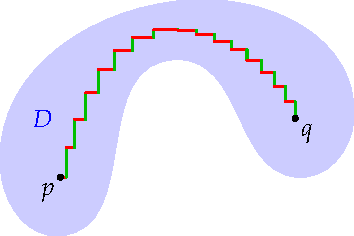
\includegraphics{analytic-topology}
\end{minipage}\medbreak
For each horizontal segment ($x_1\le x\le x_2$, $y$ fixed), we apply the mean value theorem to the functions $x\mapsto u(x,y)$ and $x\mapsto v(x,y)$. We therefore have $\widehat x,\widetilde x\in (x_1,x_2)$ with
\[\frac{u(x_2,y)-u(x_1,y)}{x_2-x_1}=u_x(\widehat x,y)=0\quad\text{and}\quad \frac{v(x_2,y)-v(x_1,y)}{x_2-x_1}=v_x(\widetilde x,y)=0\]
whence $u$ and $v$, and thus $f(z)$, are constant along any horizontal segment.\smallbreak
The same holds along any vertical segment, this time after utilizing the fact that $u_y=v_y=0$.\smallbreak
 We conclude that $f(q)=f(p)$: since $p,q$ were arbitrary points of $D$, $f$ is constant.\hfill\qedsymbol
\end{tcolorbox}
\goodbreak

% \begin{proof}
% Any two points in $D$ may be joined via a path comprising finitely many horizontal and vertical segments.\par
% \begin{minipage}[t]{0.6\linewidth}\vspace{0pt}
% Since $f'(z)=u_x+iv_x=u_y-iv_y=0$, we see that all four partial derivatives are zero.\\
% For a horizontal segment ($x_1\le x\le x_2$, $y$ fixed), the mean value theorem says $\exists \hat x\in (x_1,x_2)$ with
% \[u(x_2,y)-u(x_1,y)=(x_2-x_1)u_x(\hat x,y)=0\]
% whence $u$ is constant along any horizontal segment. The same holds for $v$, and similarly for both along any vertical segment.
% \end{minipage}\begin{minipage}[t]{0.4\linewidth}\vspace{0pt}
% \flushright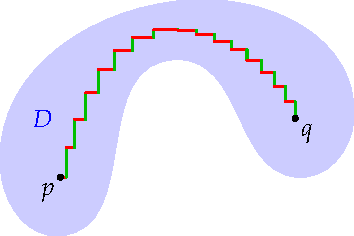
\includegraphics{analytic-topology}
% \end{minipage}\par
% We conclude that $u,v$ take the same values at any two points in $D$.
% \end{proof}



\begin{cor}{}{modimpliesconst}
If $f(z)$ is holomorphic and $\nm{f(z)}$ is constant, then $f(z)$ is constant. 
\end{cor}

This is essentially trivial in the real case: think about why! In the complex case, we need a proof.

\begin{proof}
Clearly $\nm{f(z)}^2=f(z)\cl{f(z)}=k$ is constant. If $k=0$, we are done. Otherwise, $\cl{f(z)}=\frac k{f(z)}$ is holomorphic (quotient rule!). Write $f(z)=u+iv$, whence $\cl{f(z)}=u-iv$, and consider the Cauchy--Riemann equations for \emph{both}:
\[u_x=v_y,\qquad u_y=-v_x,\qquad u_x=-v_y,\qquad u_y=v_x\]
We conclude that all partial derivatives are zero: $f'(z)=0$ and so $f$ is constant.
\end{proof}

We now come to a significant contrast with the real case. 

\begin{thm}{}{holoinfdiff}
If $f(z)=u+iv$ is holomorphic, then $f$ is \emph{infinitely differentiable.} Otherwise said:
\begin{itemize}
  \item $f^{(n)}(z)$ exists and is continuous for all $n\in\N$.
  \item $u$ and $v$ have continuous partial derivatives of all orders.
\end{itemize} 
\end{thm}

In real analysis, even functions which are differentiable everywhere need not be \emph{twice} differentiable, let alone infinitely so (Exercise \ref{exs:realoncediff}). We'll prove this important result later in the course once we've developed some integration theory.

\boldinline{Harmonic Functions}

We may now consider what happens with the \emph{second} partial derivatives of a holomorphic function:
\[u_{xx}=\partials xu_x\overset{CR1}{=}\partials xv_y =v_{yx}\overset{(\ast)}{=}v_{xy}=\partials yv_x\overset{CR2}{=}-\partials yu_y=-u_{yy}\]
Equality of the mixed partial derivatives $(\ast)$ follows because all derivatives are continuous (Theorem \ref{thm:holoinfdiff} and Clairaut's Theorem). The same equation holds for $v$. We conclude:

\begin{cor}{}{}
If $f=u+iv$ is holomorphic, then $u$ and $v$ are \emph{harmonic functions}; solutions to \emph{Laplace's equation}
\[\nabla^2u=u_{xx}+u_{yy}=0\]
\end{cor}

Laplace's equation is one of the most important partial differential equations, and is widely used throughout mathematics and physics.

\begin{example}{}{}
$f(z)=\frac 1z=\frac{x-iy}{x^2+y^2}$ is holomorphic on $\C\setminus\{0\}$; its real and imaginary parts are therefore harmonic away from the origin. Indeed,
\begin{align*}
u_{xx}+u_{yy}&=\left(\partials[^2]{x^2}+\partials[^2]{y^2}\right)\frac x{x^2+y^2} =\partials x\frac{y^2-x^2}{(x^2+y^2)^2}-\partials y\frac{2xy}{(x^2+y^2)^2}\\
&=\frac{-2x(x^2+y^2)-4x(y^2-x^2)}{(x^2+y^2)^3}-\frac{2x(x^2+y^2)-8xy^2}{(x^2+y^2)^3} =0
\end{align*}
\end{example}
\goodbreak

\boldinline{Analytic Continuations}

Though we cannot yet prove it, now is a good time to introduce another surprising property of holomorphic/analytic functions. Since this result will be seen to depend on power series, we'll stick to using the term \emph{analytic} here. 

\begin{thm}[lower separated=false, sidebyside, sidebyside align=top seam, sidebyside gap=0pt, righthand width=0.38\linewidth]{}{analyticcont}
Suppose that $f$ and $g$ are analytic functions on an open connected domain $D$ and assume that \textcolor{red}{$f(z)=g(z)$} on some \textcolor{red}{path} contained in $D$.\smallbreak
Then \textcolor{blue}{$f(z)=g(z)$} throughout $D$.
\tcblower
\flushright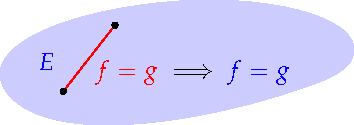
\includegraphics{analytic-topology2}
\end{thm}

This is highly counter-intuitive; you need only know the values of an analytic function on a tiny path to know the full function on its whole (connected) domain! This leads to a new concept.

\begin{defn}[lower separated=false, sidebyside, sidebyside align=top seam, sidebyside gap=0pt, righthand width=0.38\linewidth]{}{}
Let $D\subseteq E$ be open connected domains and $g:E\to \C$ an analytic function. Let $f:D\to\C$ be the restriction of $g$ to $D$; that is $f(z)=g(z)$ on $D$.\smallbreak
We call $g$ \emph{the analytic continuation} of $f$ to $E$.\tcblower
\flushright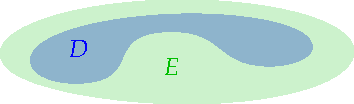
\includegraphics{analytic-topology3}
\end{defn}

By Theorem \ref{thm:analyticcont}, the analytic continuation of $f$ to $E$ must be unique. There are, however, some subtleties, which we explore a little in the next example:
\begin{itemize}\itemsep2pt
  \item Given $f$ analytic on $D$ and $D\subseteq E$, an analytic continuation is not guaranteed to exist.
  \item The choice of extended domain $E$ \emph{really} matters.
\end{itemize}

\begin{example}{}{sqrtzanalcont}
Consider the principal square root $f(z)=\sqrt z=\sqrt r\polar{i\theta}2$ with domain $D$ the first quadrant. In Exercise \ref{exs:sqrtzdiff}, we'll see that $f$ is differentiable on $D$.\smallbreak
Consider two analytic continuations of $f$: in both cases we use the same formula $z\mapsto\sqrt r\polar{i\theta}2$ and we distinguish the point $w=\polarn{3\pi i}4=\polar{5\pi i}4$ for comparison.\par
\begin{minipage}[t]{0.59\linewidth}\vspace{-5pt}
Let $G=\C\setminus\{-x:x\in\R^+_0\}$ be the plane omitting the \emph{non-positive real axis} and let
\[g:G\to\C:z\mapsto \sqrt r\polar{i\theta}2,\quad \theta=\Arg z\in(-\pi,\pi)\]
The codomain of $g$ is the right half-plane and $g(w)=\polarn{3\pi i}8$ lies in the \emph{fourth quadrant.}\medbreak
Let $H=\C\setminus\{-iy:y\in\R^+_0\}$ omit the \emph{non-positive imaginary axis} and let
\[h:H\to\C:z\mapsto \sqrt r\polar{i\theta}2,\quad \theta=\arg z\in(-\tfrac\pi 2,\tfrac{3\pi}2)\]
This time the codomain of $h$ is the upper-right half-plane; moreover $h(w)=\polar{5\pi i}8=-g(w)$ lies in the \emph{second quadrant.}
\end{minipage}\begin{minipage}[t]{0.41\linewidth}\vspace{-15pt}
\flushright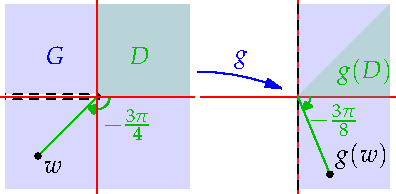
\includegraphics{analytic-cont1}\\
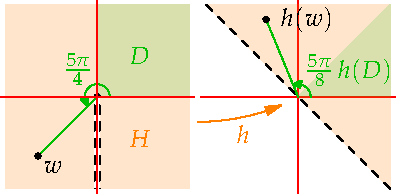
\includegraphics{analytic-cont2}
\end{minipage}\smallbreak
We have two analytic continuations of $f$ which disagree on the intersection of their domains!\smallbreak
It can moreover be seen that the omissions chosen for $G,H$ are necessary: there is no analytic continuation of $f$ to the punctured plane $\C\setminus\{0\}$, or indeed to any domain in which it is possible to loop completely around the origin. We shall return to this topic later\ldots
\end{example}
\goodbreak

% \subsubsection*{The Cauchy--Riemann Equations in Polar Co-ordinates}
% 
% Recall that $z=x+iy=re^{i\theta}$, where $x=r\cos\theta$ and $y=r\sin\theta$, we may apply the chain rule to see that
% \[u_r=u_xx_r+u_yy_r =u_x\cos\theta-u_y\sin\theta \qquad u_\theta=u_xx_\theta+u_yy_\theta =-u_xr\sin\theta +u_yr\cos\theta\]
% with similar expressions for $v_x,v_y$. Comparing to Theorems \ref{thm:cauchyriemann} and \ref{thm:cauchyriemann2}, we quickly obtain the corresponding results in polar co-ordinates:

\vfill\goodbreak

\begin{exercises*}{}
\hangindent\leftmargini
\textup{1.}\ Suppose $g'(z)=h'(z)$  on an open connected domain $D$. Prove that $h(z)=g(z)+c$ for some constant $c\in\C$.\vspace{-5pt}
\begin{enumerate}\setcounter{enumi}{1}
  \item[](\emph{Equivalently: if $g(z)$ and $h(z)$ are anti-derivatives of $f(z)$ on an open connected domain $D$ then $g(z)-h(z)$ is constant on $D$.})
  
  \item Check explicitly that $u=e^{nx}\cos ny$ and $v=e^{nx}\sin ny$ are harmonic functions for any $n\in\Z$.
  
  \item Prove or disprove: if $u,v:D\to\R$ are harmonic functions on an open set $D\subseteq\R^2$, then $f(z):=u(x,y)+iv(x,y)$ is holomorphic.
  
  \item\label{exs:realoncediff} Define $f:\R\to\R$ by
	\[f(x)=x\nm x=\begin{cases}
		x^2&\text{if }x\ge 0\\
		-x^2&\text{if }x<0
		\end{cases}\]
		Show that $f$ is differentiable, but not \emph{twice} differentiable.\par
		(\emph{Such properties are impossible for complex functions})
% 		\footnote{Perhaps this isn't such a surprise: as we saw in Example \hyperref[exs:modnotdiff]{\ref*{ex:crlots}.\ref*{exs:modnotdiff}}, corresponding functions of the complex numbers (using the modulus) aren't differentiable at all!}
  
  \item\label{exs:crpolar} Suppose $f(z)=u+iv$ and write $z=x+iy=re^{i\theta}$ in polar form.
  \begin{enumerate}
    \item Use the chain rule applied to the polar co-ordinate relations
  	\[x=r\cos\theta,\qquad y=r\sin\theta\]
  	to compute the partial derivatives $u_r,u_\theta,v_r$ and $v_\theta$.
  	\item Deduce the polar form of the Cauchy--Riemann equations:
		\[ru_r=v_\theta\qquad u_\theta=-rv_r,\qquad f'(z)=e^{-i\theta}(u_r+iv_r) =\frac{-i}{z}(u_\theta+iv_\theta)\]
	\end{enumerate}
	
	\item Prove the polar form of Laplace's equation:
	\[r^2u_{rr}+ru_r+u_{\theta\theta}=0\]
		
	\item Show that $u=r^n\cos n\theta$ is a harmonic function for any $n\in\N$: find \emph{two} ways to show that this is true!
	
	
	\item Suppose $f:\C\to\C$ is an entire function such that $f(iy)=-iy^3$ whenever $z=iy$ lies on the imaginary axis. What is the value $f(2)$? Explain your answer.
	
	\item The function $f(z)=\frac 1z$ is analytic on $\C\setminus\{0\}$. Explain why there is no analytic continuation of $f$ that is analytic at $z=0$.
	
	\item\label{exs:sqrtzdiff}
	\begin{enumerate}
	  \item Use Exercise \ref{exs:crpolar} to prove that $f(z)=\sqrt z=\sqrt r\polar{i\theta}2$ is analytic on the first quadrant, and find $f'(z)$. Moreover, explain why the functions $g, h$ in  Example \ref{ex:sqrtzanalcont} are analytic and therefore analytic continuations of $f$.
	  \item Prove that there exists no analytic continuation of $g$ to any set larger than $G$.\\
		(\emph{Hint: suppose the extended domain contains $-r\in\R^-$. Now use the fact that an analytic continuation must be continuous at $-r\ldots$})
	\end{enumerate}
\end{enumerate}
\end{exercises*}